% 第 5 章
\section{另一个不动点：当 $d > n$ 时梯度下降去向何处}\label{sec:gd-underdet}

第 \ref{sec:gd} 章的精确解 \eqref{eq:gd-exact} 有一个隐藏前提：$\X^\top\X$ 可逆。本章转向相反的\textbf{欠定}（underdetermined）情形 $d > n$：方程个数少于未知数，$\X^\top\X \in \R^{d \times d}$ 必奇异（秩 $\le n < d$），闭式解 \eqref{eq:ols-closed} 不复存在，第 \ref{sec:gd} 章的衰减矩阵 $\bm{I} - \eta\X^\top\X$ 有 $d - n$ 个特征值恒等于 $1$——误差在某些方向上\textbf{永不衰减}。然而正是在这里，gradient descent 给出了一个深刻的结果：\textbf{迭代依然收敛，只是收敛到一个由初值选定的特殊解；从 $\widehat{\bbeta}_0 = \zero$ 出发，它收敛到最小范数解}
\[
  \widehat{\bbeta}' = \X^\top (\X \X^\top)^{-1} \y .
\]

\subsection{设定：$d > n$，解已成流形}\label{sec:underdet-setup}

设 $\X \in \R^{n \times d}$ \textbf{行满秩}（$\rank(\X) = n$，即 $n$ 行线性无关；连续分布的随机数据几乎必然如此），则 $\X\X^\top \in \R^{n \times n}$ 对称正定、可逆。此时：

\begin{itemize}
  \item 方程组 $\X \bbeta = \y$ \textbf{相容}（$\y$ 必在列空间内），且解\textbf{不唯一}：通解为
  \[
    \big\{ \bbeta : \X \bbeta = \y \big\} = \widehat{\bbeta}' + \mathcal{N}(\X),
    \qquad
    \mathcal{N}(\X) = \{ \bm{w} \in \R^d : \X \bm{w} = \zero \},
  \]
  一个 $d - n$ 维的仿射子空间（解流形）——每个点都是一个插值解；
  \item 损失 $L(\bbeta) = \frac{1}{2}\norm{\y - \X\bbeta}^2$ 在该流形上恒为零，即全局最小值为 $0$ 且\textbf{在一个流形上取到}；
  \item $\X^\top\X$ 有 $d - n$ 个零特征值，$(\X^\top\X)^{-1}$ 无定义——第 \ref{sec:gd} 章的全部公式在此处失效。
\end{itemize}

\subsection{一个新的不动点及其两个验证}

\subsubsection*{验证 1：精确插值}
直接代入：
\begin{equation}\label{eq:interp}
  \X \, \widehat{\bbeta}' = \X \X^\top (\X \X^\top)^{-1} \y = \y .
\end{equation}
即 $y = \X \widehat{\bbeta}'$：训练误差精确为零——\textbf{插值}（interpolation）。这正是 $d = n$ 时「残差为零」现象（第 \ref{sec:hd-break} 节）在 $d > n$ 时的延续：模型容量过剩，拟合变成了记忆。

\subsubsection*{验证 2：一阶平衡点}
梯度为
\begin{equation}\label{eq:grad-at-p}
  \nabla L(\widehat{\bbeta}') = \X^\top \big( \X \widehat{\bbeta}' - \y \big) = \X^\top ( \y - \y ) = \zero .
\end{equation}
即 $\widehat{\bbeta}'$ 是 least-square 损失的一个\textbf{一阶平衡点}（驻点）；由 $L$ 凸且 $L(\widehat{\bbeta}') = 0 = \min L$，它其实还是全局最小点。于是它也是 GD 迭代 \eqref{eq:gd} 的不动点：$\widehat{\bbeta}' - \eta\, \nabla L(\widehat{\bbeta}') = \widehat{\bbeta}'$ 对\textbf{任意} $\eta$ 成立。事实上由 \eqref{eq:grad-at-p} 可见：\textbf{整个解流形 $\widehat{\bbeta}' + \mathcal{N}(\X)$ 上的每一点都是不动点}——这不是一个孤立的平衡点，而是一整个平衡点集合。

\subsection[最小范数性：解流形上离原点最近的点]{最小范数性：$\widehat{\bbeta}'$ 是解流形上离原点最近的点}\label{sec:minnorm}

\begin{theorem}[最小范数解]\label{thm:minnorm}
在解流形 $\{ \bbeta : \X \bbeta = \y \}$ 上，$\widehat{\bbeta}' = \X^\top(\X\X^\top)^{-1}\y$ 是唯一的 Euclidean 范数最小点。
\end{theorem}
\begin{proof}
任取解 $\bbeta$，写 $\bbeta = \widehat{\bbeta}' + \bm{w}$，其中 $\X\bm{w} = \zero$（两解之差在零空间内）。关键观察：$\widehat{\bbeta}' \perp \mathcal{N}(\X)$，因为
\[
  \langle \widehat{\bbeta}',\ \bm{w} \rangle = \y^\top (\X\X^\top)^{-1} \X\, \bm{w} = 0 .
\]
于是由勾股定理
\[
  \norm{\bbeta}^2 = \norm{\widehat{\bbeta}'}^2 + \norm{\bm{w}}^2 \;\ge\; \norm{\widehat{\bbeta}'}^2,
\]
等号当且仅当 $\bm{w} = \zero$。$\widehat{\bbeta}'$ 正是解流形在 row$(\X)$（$\X^\top$ 的列空间）上的那个点。
\end{proof}

\subsection{稳定性：行空间收缩，零空间中性}\label{sec:stability}

不动点集合那么大，迭代到底收不收敛、收敛到哪？把第 \ref{sec:gd} 章的稳定性分析搬过来，只换特征谱。GD 映射 $\bm{G}(\bbeta) = \bbeta - \eta \nabla L(\bbeta)$ 的线性化（它本身就是线性的）为
\[
  \bm{G}(\bbeta) - \bm{G}(\bbeta_0) = (\bm{I} - \eta \X^\top \X)(\bbeta - \bbeta_0).
\]
$\X^\top\X$ 的特征值：$n$ 个正特征值 $\lambda_1 \ge \dots \ge \lambda_n > 0$（与 $\X\X^\top$ 的非零特征值完全相同），外加 $d - n$ 个 $0$。于是 $\bm{I} - \eta\X^\top\X$ 的特征值为
\[
  \underbrace{1 - \eta \lambda_j}_{n \text{ 个}},\ j = 1..n;
  \qquad
  \underbrace{1}_{d - n \text{ 个}}.
\]
\begin{itemize}
  \item \textbf{行空间方向}（$d - n$ 个零特征值对应方向的正交补）：当 $0 < \eta < \dfrac{2}{\lambda_{\max}(\X\X^\top)}$ 时 $|1 - \eta\lambda_j| < 1$——\textbf{收缩}，与 $n \gg d$ 情形完全相同的指数衰减；
  \item \textbf{零空间方向}：因子恒为 $1$——\textbf{中性}：初始误差中的 $\mathcal{N}(\X)$ 分量\textbf{原样保留，永不衰减}。
\end{itemize}

结论分层说清楚：
\begin{enumerate}[label=(\arabic*)]
  \item 解流形 $\widehat{\bbeta}' + \mathcal{N}(\X)$ 上的\textbf{每一个点都是 Lyapunov 稳定}的：横向（行空间）扰动被指数压回流形附近，切向（零空间）扰动既不放大也不消失，迭代始终停留在扰动点的有界邻域内；
  \item 作为\textbf{孤立的点}，流形上的每个平衡点都不是渐近稳定的（切向的小扰动不会回来）——稳定的是\textbf{流形本身}：它是横向吸引的（normally attracting）；
  \item \textbf{初值决定落点}：由于零空间分量守恒，$\widehat{\bbeta}_0$ 的零空间分量被一路携带到极限——
  \[
    \lim_{t \to \infty} \widehat{\bbeta}_t = \widehat{\bbeta}' + \underbrace{\bm{P}_{\mathcal{N}(\X)}\, \widehat{\bbeta}_0}_{\text{零空间分量}} ,
  \]
  其中 $\bm{P}_{\mathcal{N}(\X)}$ 是到零空间的正交投影。
\end{enumerate}

\subsection{精确解（续）：GD 从零点出发 = 隐式最小范数正则化}\label{sec:implicit}

取最常见的初值 $\widehat{\bbeta}_0 = \zero$：零空间分量为零，于是迭代的\textbf{全程都待在 row$(\X)$ 里}（归纳可见 $\widehat{\bbeta}_t = \X^\top \bm{u}_t$ 对某 $\bm{u}_t$ 成立，因为梯度 $\X^\top(\cdot)$ 总把向量拉回行空间）。行空间里只有一个插值点——就是 $\widehat{\bbeta}'$。于是：

\begin{theorem}[欠定情形的 GD 精确解]\label{thm:gd-exact-underdet}
设 $\X$ 行满秩，$0 < \eta < 2/\lambda_{\max}(\X\X^\top)$，$\widehat{\bbeta}_0 = \zero$。则
\begin{equation}\label{eq:gd-exact-underdet}
  \boxed{\;\widehat{\bbeta}_t = \Big[ \bm{I} - \big( \bm{I} - \eta\, \X^\top \X \big)^{t} \Big]\, \X^\top (\X \X^\top)^{-1} \y
       = \Big[ \bm{I} - \big( \bm{I} - \eta\, \X^\top \X \big)^{t} \Big]\, \widehat{\bbeta}'\;}
\end{equation}
且 $\widehat{\bbeta}_t \to \widehat{\bbeta}'$（最小范数插值解），收敛率由 $\X\X^\top$ 的条件数决定：$\norm{\widehat{\bbeta}_t - \widehat{\bbeta}'} = O\big( \big(\frac{\kappa - 1}{\kappa + 1}\big)^t \big)$（在最优步长下）。
\end{theorem}
\begin{proof}
用恒等式 $\X^\top (\bm{I} - \eta \X\X^\top) = (\bm{I} - \eta \X^\top\X) \X^\top$（两边都等于 $\X^\top - \eta \X^\top \X \X^\top$）对 \eqref{eq:gd} 递推，得 $\widehat{\bbeta}_t = \X^\top \big[ \eta \sum_{k=0}^{t-1} (\bm{I} - \eta\X\X^\top)^k \big] \y$。括号内是 $\R^{n \times n}$ 上的几何级数，$\eta < 2/\lambda_{\max}$ 保证其谱半径小于 $1$（全部特征严格收缩），于是 $\eta \sum_{k<t}(\bm{I} - \eta\X\X^\top)^k = \big[ \bm{I} - (\bm{I} - \eta\X\X^\top)^t \big](\X\X^\top)^{-1}$，代回并再次使用上述恒等式即得 \eqref{eq:gd-exact-underdet}。极限由 $(\bm{I} - \eta\X\X^\top)^t \to \zero$ 给出；收敛率照搬推论 \ref{thm:gd-opt}，只是把 $\X^\top\X$ 的谱换成 $\X\X^\top$ 的谱（非零特征值相同）。
\end{proof}

把 \eqref{eq:gd-exact-underdet} 与 \eqref{eq:gd-exact-zero} 并排看，结构完全一致——\textbf{唯一的差别是「目标点」从 $\bhat = (\X^\top\X)^{-1}\X^\top\y$ 换成了 $\widehat{\bbeta}' = \X^\top(\X\X^\top)^{-1}\y$}。形式上的对称绝非巧合，下一节给出统摄两者的对象。

\begin{remark}[隐式正则化]
定理 \ref{thm:gd-exact-underdet} 是现代「隐式正则化 / 隐式偏差」（implicit regularization / implicit bias）理论的原型：\textbf{没有任何显式惩罚项，单纯从零点做梯度下降，就自动选出了所有插值解中范数最小、因而往往最泛化的那一个}。过参数化神经网络在训练中「不爆记忆、反而泛化」的现象，其最干净的数学化身就是这个线性版本。
\end{remark}

\begin{figure}[htbp]
  \centering
  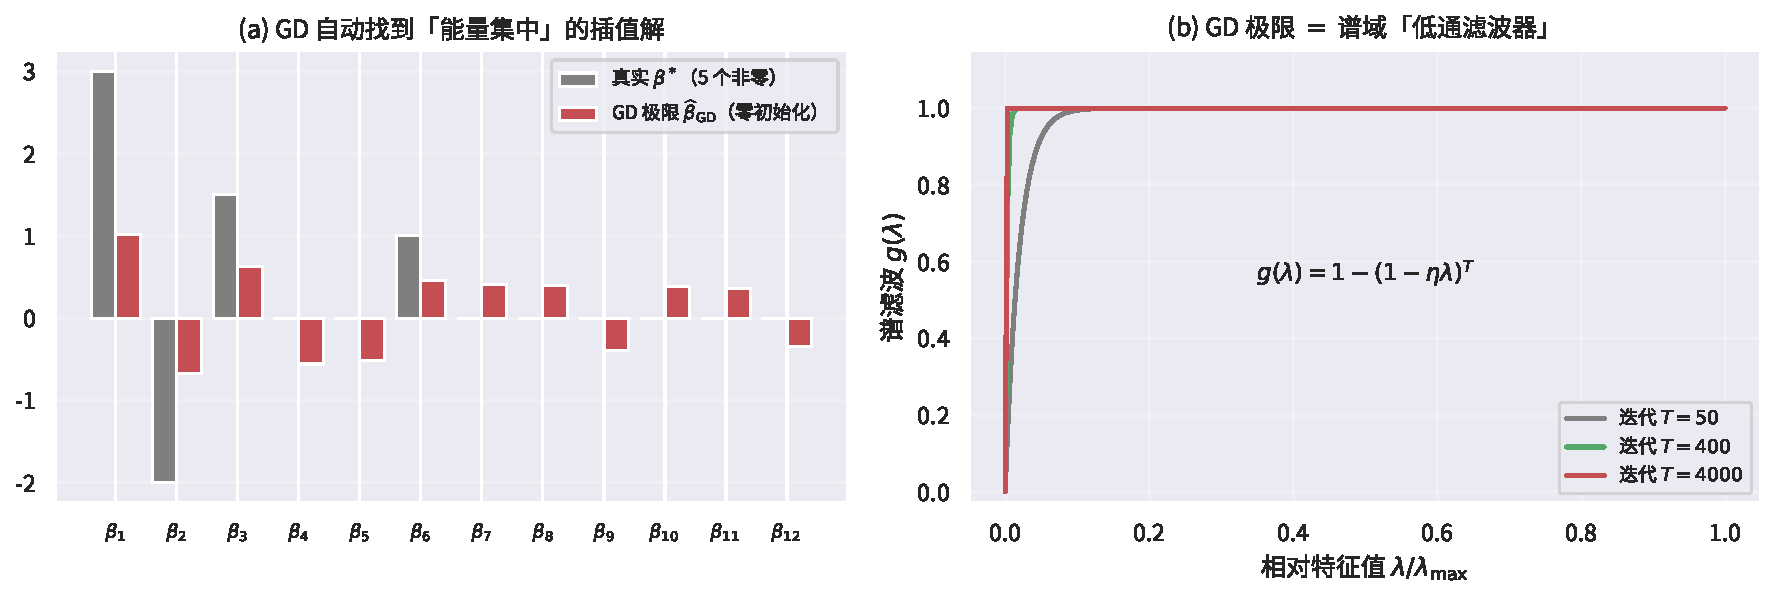
\includegraphics[width=\linewidth]{figures/ch5_implicit.pdf}
  \caption{隐式正则化的两个面孔（$d=100>n=30$，无噪声插值）：(a) 零初始化 GD 的极限（红）在真实信号方向（灰，5 个非零系数）上恢复能量、在噪声方向自动收缩；(b) 谱滤波解释——$t$ 步 GD 在特征方向 $\lambda$ 上施加因子 $g(\lambda)=1-(1-\eta\lambda)^t$，大特征方向先收敛、小特征方向后收敛，等效于一个「低通滤波器」。}
  \label{fig:ch5-implicit}
\end{figure}

\subsection{与伪逆解的比较：一个对象，几张面孔}\label{sec:pseudo-compare}

现在回答本章的比较问题。Moore--Penrose 伪逆 $\X^+$ 由 SVD 统一定义：若 $\X = \bm{U} \bm{\Sigma} \bm{V}^\top$（$\bm{\Sigma}$ 对角、元为奇异值 $s_j > 0$），则
\[
  \X^+ = \bm{V} \bm{\Sigma}^{+} \bm{U}^\top, \qquad
  \bm{\Sigma}^{+} \text{ 把每个 } s_j \text{ 换成 } 1/s_j \ (\text{零保持不变}).
\]
它给出\textbf{任意} $\X$ 的\textbf{最小范数最小二乘解} $\X^+\y$。两个秩情形分别退化为两个熟悉的公式：

\begin{itemize}
  \item \textbf{列满秩}（$n \gg d$）：$\X^+ = (\X^\top\X)^{-1}\X^\top$——第 \ref{sec:hd-closed} 节的 OLS 闭式解；
  \item \textbf{行满秩}（$d > n$）：$\X^+ = \X^\top(\X\X^\top)^{-1}$——\textbf{正是本节的 $\widehat{\bbeta}'$}。（代入 SVD 即可验证：$\X\X^\top = \bm{U}\bm{\Sigma}\bm{\Sigma}^\top\bm{U}^\top$，逆为 $\bm{U}(\bm{\Sigma}\bm{\Sigma}^\top)^{-1}\bm{U}^\top$，左乘 $\X^\top = \bm{V}\bm{\Sigma}^\top\bm{U}^\top$ 得 $\bm{V}\bm{\Sigma}^+\bm{U}^\top$。）
\end{itemize}

所以：\textbf{在 $d > n$ 行满秩时，$\widehat{\bbeta}'$ 就是伪逆解}——不是「另一个解」，而是同一对象在欠定 regime 的面孔。下表把全文出现的所有「同一个点」的到达方式收拢：

\begin{center}
\resizebox{\linewidth}{!}{%
\begin{tabular}{@{}llll@{}}
\toprule
对象 & 公式 & 适用 & 到达方式 \\
\midrule
OLS 闭式解 & $(\X^\top\X)^{-1}\X^\top\y$ & $n \gg d$ 列满秩 & 直接解正规方程 \\
\textbf{本章 $\widehat{\bbeta}'$} & $\X^\top(\X\X^\top)^{-1}\y$ & $d > n$ 行满秩 & 直接解插值方程 \\
伪逆解 $\X^+\y$ & SVD 定义 & 任意秩 & 统一定义（上两者的母对象） \\
GD，$\widehat{\bbeta}_0 = \zero$ & $\lim_t \widehat{\bbeta}_t$ & 任意秩 & 隐式收敛到 $\X^+\y$（本两章精确解） \\
ridge，$\lambda \to 0^+$ & $\lim_{\lambda \to 0^+}(\X^\top\X + \lambda\bm{I})^{-1}\X^\top\y$ & 任意秩 & 同 $\X^+\y$（恒等式取极限，见练习） \\
\bottomrule
\end{tabular}}
\end{center}

两点比较结论值得单独记住：

\begin{enumerate}[label=(\arabic*)]
  \item \textbf{代数上}：$\widehat{\bbeta}' = \X^+\y$（行满秩时）——它与伪逆解\textbf{完全相同}，包括那条「最小范数」性质：伪逆的全部定义性质中，$\X^+\y \perp \mathcal{N}(\X)$ 这一条在欠定情形正是定理 \ref{thm:minnorm} 的内容。
  \item \textbf{动力学上}：伪逆是「静态」的（SVD 一刀切出答案），GD 是「动态」的（多项式一步步逼近）：\eqref{eq:gd-exact-underdet} 显示 GD 的 $t$ 步解 $= \big[\bm{I} - (\bm{I} - \eta\X^\top\X)^t\big]\X^+\y$，括号内是作用在伪逆解上的收缩多项式。换一个初值，GD 还会走到\textbf{别的}插值点（带上初值的零空间分量）——\textit{GD 族抵达的是整个解流形，伪逆（以及零点初值）选中的是流形上离原点最近的那一点}。
\end{enumerate}

\begin{keybox}[本章要点]
\begin{itemize}
  \item $d > n$ 行满秩时 $\widehat{\bbeta}' = \X^\top(\X\X^\top)^{-1}\y$ 满足 (i) 精确插值 $\X\widehat{\bbeta}' = \y$、(ii) $\nabla L(\widehat{\bbeta}') = \zero$（一阶平衡点），且是解流形上\textbf{唯一的最小范数}点；
  \item 整个解流形 $\widehat{\bbeta}' + \mathcal{N}(\X)$ 都是 GD 的不动点：行空间方向（$0 < \eta < 2/\lambda_{\max}(\X\X^\top)$ 时）指数收缩，零空间方向中性——流形横向吸引、点仅 Lyapunov 稳定，落点由初值的零空间分量决定；
  \item 精确解 $\widehat{\bbeta}_t = [\bm{I} - (\bm{I} - \eta\X^\top\X)^t]\widehat{\bbeta}'$：与 $n \gg d$ 情形结构同构，目标点由 $\bhat$ 换成 $\widehat{\bbeta}'$；$\widehat{\bbeta}_0 = \zero$ 时 GD \textbf{隐式}收敛到最小范数解——隐式正则化的线性原型；
  \item 与伪逆的关系：行满秩时 $\widehat{\bbeta}' = \X^+\y$ 恒等；伪逆、两个闭式公式、GD 零点极限、ridge 零极限是\textbf{同一个最小范数最小二乘解}的五张面孔。
\end{itemize}
\end{keybox}

\begin{exercise}\label{ex:ridge-dual}
证明恒等式 $(\X^\top\X + \lambda\bm{I})^{-1}\X^\top = \X^\top(\X\X^\top + \lambda\bm{I})^{-1}$（两边同乘 $(\X^\top\X + \lambda\bm{I})$ 并整理），并由此说明 ridge 解在 $\lambda \to 0^+$ 时收敛到 $\X^+\y$（无需满秩假设）。
\end{exercise}

\begin{exercise}\label{ex:gd-limit-anyinit}
设 $d > n$、$\X$ 行满秩。证明：对任意初值 $\widehat{\bbeta}_0$，GD 的极限为 $\widehat{\bbeta}' + \bm{P}_{\mathcal{N}(\X)} \widehat{\bbeta}_0$，其中 $\bm{P}_{\mathcal{N}(\X)} = \bm{I} - \X^+\X$ 是到零空间的正交投影；并解释为何这一结论与定理 \ref{thm:gd-exact-underdet} 一致。
\end{exercise}

\begin{exercise}\label{ex:spectrum}
对比两个 regime 的「有效维数」：$n \gg d$ 时 GD 误差衰减由 $\X^\top\X$ 的 $d$ 个特征值决定；$d > n$ 时由 $\X\X^\top$ 的 $n$ 个特征值决定。证明两矩阵的非零特征值完全相同（提示：若 $\X^\top\X \bm{v} = \lambda \bm{v}$，考察 $\X \bm{v}$），并解释这一谱同一性为何使两章的收敛率公式可以互换。
\end{exercise}
